\documentclass[oneside,a4paper,14pt]{extarticle}
\usepackage[a4paper,letterpaper,top=20mm,bottom=20mm,left=20mm,right=10mm]{geometry}
\usepackage[russian]{babel}
\usepackage{indentfirst}
\usepackage{amsmath}
\usepackage{amsfonts}
\usepackage{amsthm}
\usepackage{graphicx}
\usepackage{caption}
\usepackage{titlesec}
\usepackage{minted, fancyvrb}

\titleformat{\section} {\normalsize\bfseries} {\thesection} {1em} {}
\titleformat{\subsection} {\normalsize\bfseries} {\thesubsection} {1em} {}
\titleformat{\subsubsection} {\normalsize\bfseries} {\thesubsection} {1em} {}
\renewcommand\baselinestretch{1.45}\normalsize
\setlength{\parindent}{1.25cm}

\begin{document}

\newpage
\thispagestyle{empty}
\begin{center}
	МИНИСТЕРСТВО НАУКИ И ВЫСШЕГО ОБРАЗОВАНИЯ РОССИЙСКОЙ ФЕДЕРАЦИИ ФЕДЕРАЛЬНОЕ ГОСУДАРСТВЕННОЕ БЮДЖЕТНОЕ ОБРАЗОВАТЕЛЬНОЕ УЧРЕЖДЕНИЕ ВЫСШЕГО ОБРАЗОВАНИЯ\\
	«ВЯТСКИЙ ГОСУДАРСТВЕННЫЙ УНИВЕРСИТЕТ»\\
	Институт математики и информационных систем\\
	Факультет автоматики и вычислительной техники\\
	Кафедра электронных вычислительных машин
\end{center}
\vspace{10mm}

\hfill
\begin{tabular}{l}
  \footnotesize Дата сдачи на проверку: \\
  \footnotesize <<\rule[-1mm]{5mm}{0.10mm}\/>>\rule[-1mm]{20mm}{0.10mm}\ 2025 г.\\
  \footnotesize Проверено: \\
  \footnotesize <<\rule[-1mm]{5mm}{0.10mm}\/>>\rule[-1mm]{20mm}{0.10mm}\ 2025 г. \\
\end{tabular}
\vfill

\begin{center}
    ИЗУЧЕНИЕ РАБОТЫ С МНОЖЕСТВАМИ\\
	Отчёт по лабораторной работе №1\\
	по дисциплине\\
	<<Дискретная математика>>\\
\end{center}
\vspace{25mm}
\noindent
\begin{tabular}{ll}
	Разработал студент гр. ИВТб-1301-05-00 & \rule[-1mm]{30mm}{0.10mm}\,/Черкасов А. А./   \\
	                                       & \hspace{8mm}\footnotesize(подпись)            \\
	Проверила преподаватель                & \rule[-1mm]{30mm}{0.10mm}\,/Пахарева И. В./ \\
	                                       & \hspace{8mm}\footnotesize(подпись)            \\
\end{tabular}

\noindent
  \begin{tabular}{lp{58mm}r}
    Работа защищена &  & <<\rule[-1mm]{5mm}{0.10mm}\/>>\rule[-1mm]{30mm}{0.10mm}\ 2025 г.
  \end{tabular}
  \vfill

\begin{center}
	Киров\\
	2025
\end{center}

\newpage\thispagestyle{plain}

\section*{Цель}

Цель работы: Изучение основ теории множеств, базовых операций над ними, разработка приложений на языке Паскаль согласно заданию.

\section*{Задание}
\begin{itemize}
	\item[$-$] Реализовать программу для выполнения заданных операций над множествами. Программа должна работать при некорректном вводе, выдавая информационное сообщение об ошибке.
	
	\begin{tabular}{|c|c|c|c|c|c|c|c|c|}
		\hline
		Вар / Множ & $A$  & $B$  & $C$  & $D$      & $E$       & $X$               & $Y$      & $K$             \\
		\hline
		27         & $\mathbb{R}$ & $\mathbb{Q}$ & $\mathbb{Z}$ & латиница & кириллица & $A \cap B \cap C$ & $E \cup D$ & $X \triangle Y$ \\
		\hline
		\end{tabular}
\end{itemize}

\section*{Решение}

Схема алгоритма решения представлена на рисунках 1.1, 1.2 и 1.3. Пример работы программы представлен на рисунках 2.1, 2.2. Исходный код решений представлен в Приложении А1.

\clearpage
\begin{figure}[H]
	\centering
	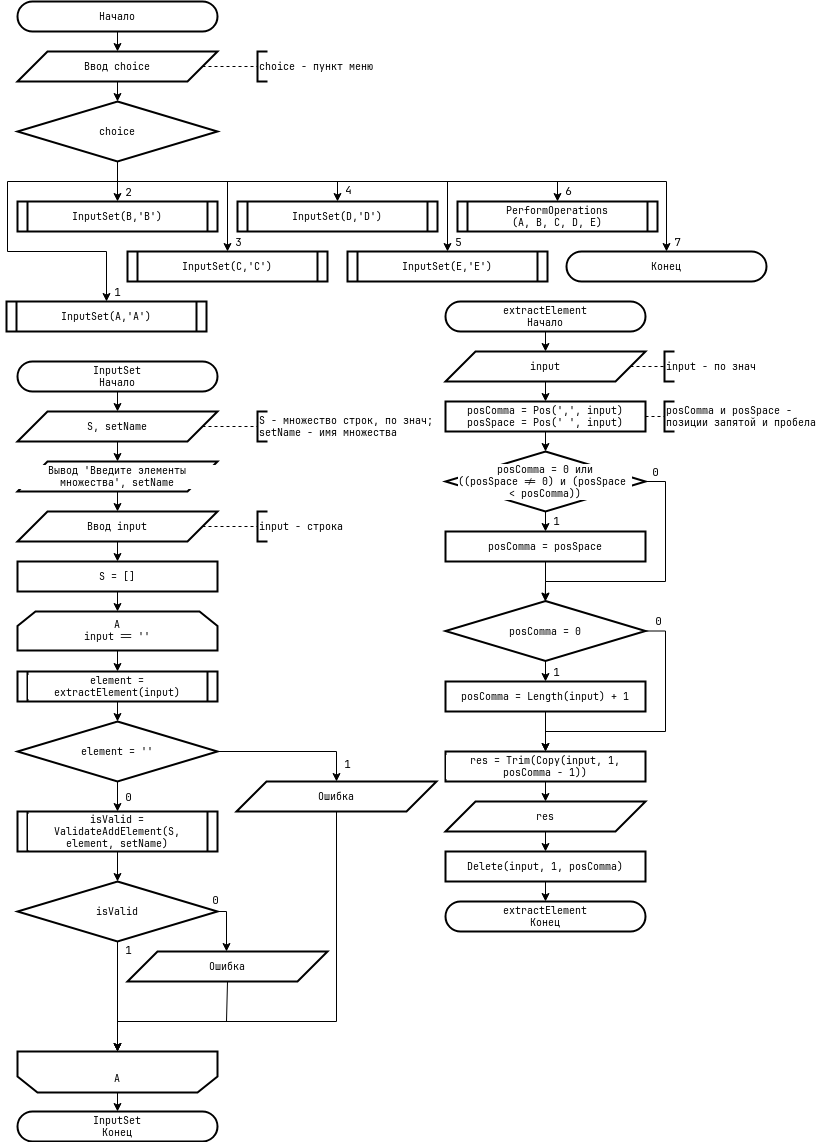
\includegraphics[height=0.9\textheight]{pics/flowchart1.png}
	\caption*{Рисунок 1.1 - Схемы алгоритмов основной программы, подпрограмм ввода множеств и извлечения элемента.}
\end{figure}

\clearpage
\begin{figure}[H]
	\centering
	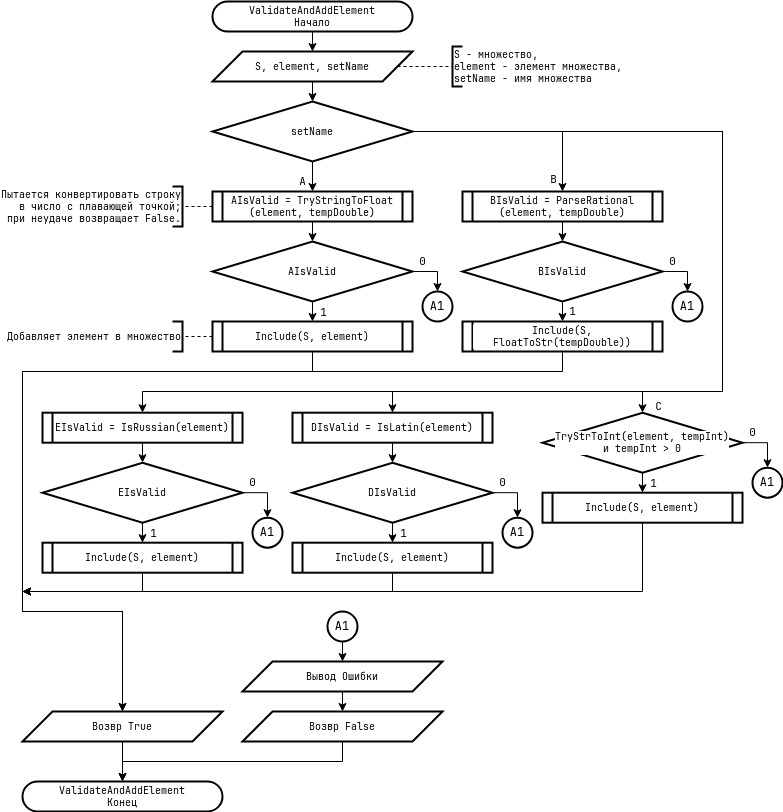
\includegraphics[width=0.9\textwidth]{pics/flowchart2.png}
	\caption*{Рисунок 1.2 - Схема алгоритма подпрограммы проверки на валидность элемента.}
\end{figure}

\clearpage
\begin{figure}[H]
	\centering
	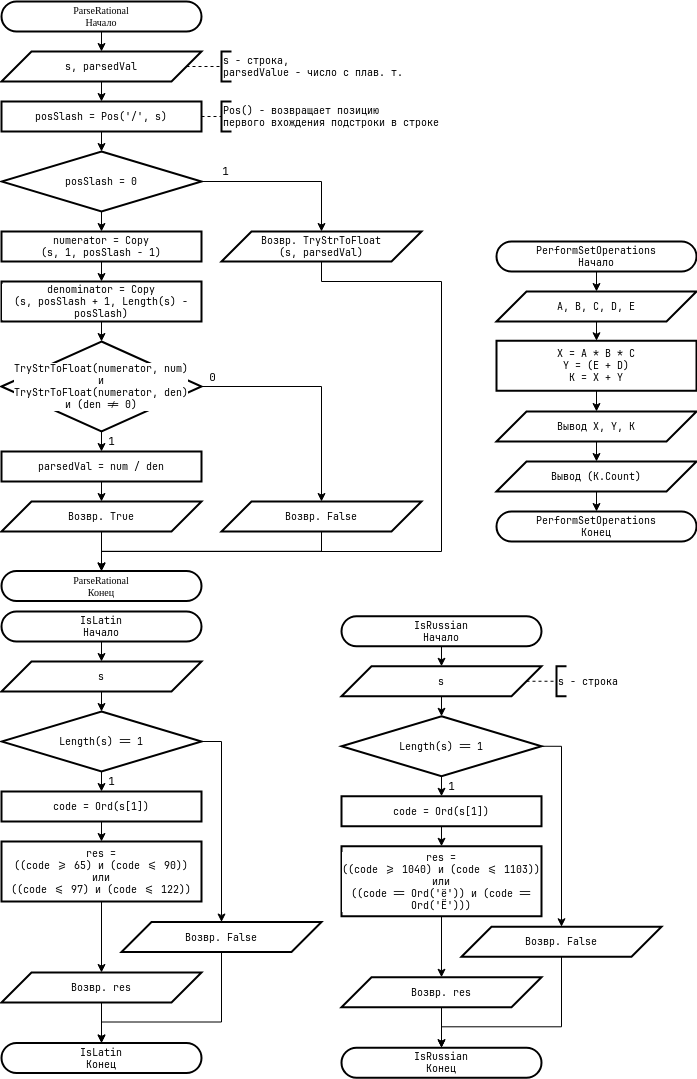
\includegraphics[height=0.9\textheight]{pics/flowchart3.png}
	\caption*{Рисунок 1.3 - Схема алгоритма подпрограмм проверки элементов на латинский и кирилличекий алфавит, подпрограмма выполнения операций с множествами.}
\end{figure}

\clearpage
\begin{figure}[H]
	\centering
	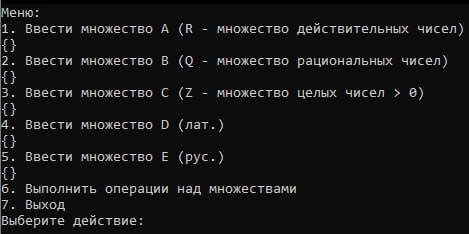
\includegraphics[width=0.9\textwidth]{pics/photo1.jpg}
	\caption*{Рисунок 2.1 - Пример работы программы.}
\end{figure}

\begin{figure}[H]
	\centering
	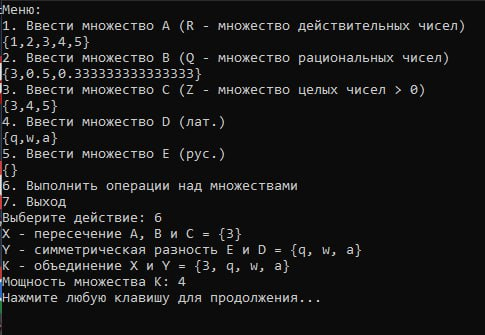
\includegraphics[width=0.9\textwidth]{pics/photo2.jpg}
	\caption*{Рисунок 2.2 - Пример работы программы.}
\end{figure}

\section*{Вывод}

\setminted{style = rainbow_dash, fontsize = \small} % https://pygments.org/styles/

В результате работы была реализованна программа выполняющая операции над множествами на языке паскаль.
\newpage
\section*{Приложение А1. Исходный код}
\inputminted{pascal}{code/main.pas}

\end{document}
